\documentclass[../main.tex]{subfiles}

\begin{document}
	\section{Structure des polymères à l'état solide}
	Comme les petites molécules, certains polymères sont cristallins. Cependant il ne sont jamais à 100\% cristallins. Les polymères qui peuvent se cristalliser sont dénommés comme \textbf{semi-cristallin}. La micro-structure des polymères semi-cristallins se compose de cristaux polymères entourés par une matrice polymères amorphe (fig. \ref{amorphe}). 
	\begin{figure}[h]
		\begin{center}
			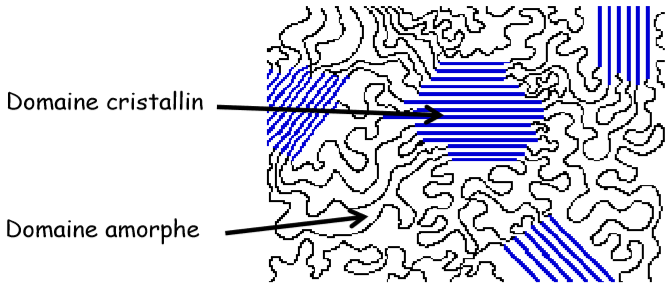
\includegraphics[scale=1]{Amorphe.png}
			\caption{\label{amorphe}Représentation des micro-structures d'un polymère semi-cristallins}
		\end{center}
	\end{figure}
	Les polymères n'ayant pas la possibilité de former des domaines cristallins se composent uniquement d'une phase amorphe et sont ainsi dénommés \textbf{polymères amorphes}.
	
	La dégradabilité ne dépend pas uniquement de la micro-structure du polymère, sa masse moléculaire ou encore sa polarité, mais ces paramètres sont souvent corrélés.
	\\
	La phase cristalline est caractérisée par un \textbf{point de fusion}, c'est à dire la température à laquelle le domaine cristallin fond. 
	
	\subsection{Phase des polymères à l'état solide}
	
	\begin{figure}[h]
		\begin{center}
			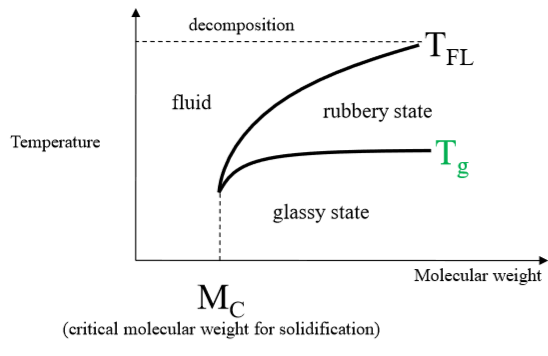
\includegraphics[scale=1]{PolyPhase.png}
			\caption{\label{polyphase}Etat d'un polymère en fonction de sa masse molécule et de sa température}
		\end{center}
	\end{figure}

	Un polymère amorphe peut généralement adopter 3 états distincts. Le nombre de phases atteignable pour un polymère ainsi que les températures de transition entre ces phases dépend de sa masse moléculaire (fig. \ref{polyphase}). 
	
	\section{Polymères amorphes vitreux}
	
	\subsection{La conformation statistique}
	\begin{figure}[h]
		\begin{center}
			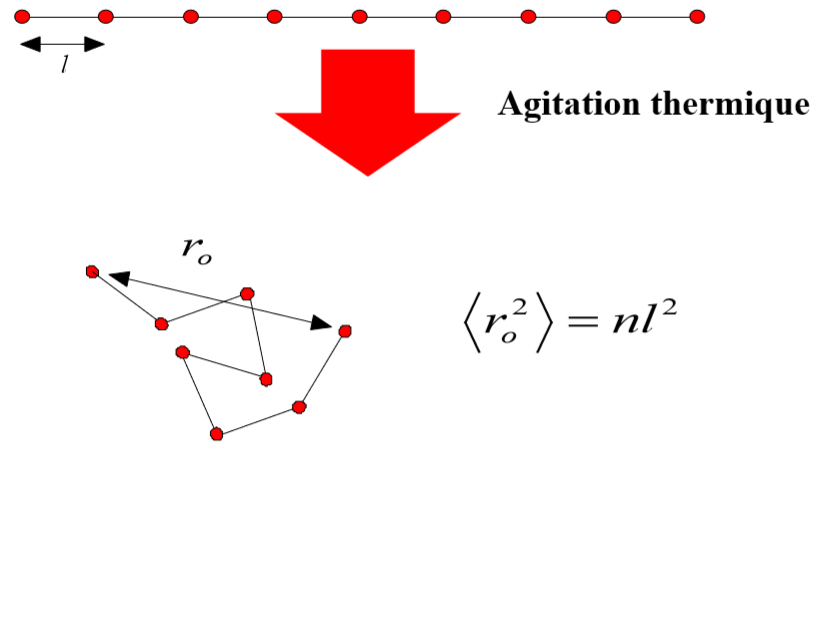
\includegraphics[width=18cm]{AmorpheVitreux.png}
			\caption{\label{amorphevitreux}Cas d'une chaîne à \textit{articulation libres} isolée}
		\end{center}
	\end{figure}

	Une chaîne isolée va adopter une conformation en \textit{pelote} statistique (qui change toutes les $10^-12$ secondes). Tel que montré sur la figure \ref{amorphevitreux}, on trouve $n$ le nombre de liaisons. $<r_0^2>$ est proportionnel à $M$. La taille d'une chaîne est proportionnelle à sa masse molaire. Pour les chaînes réelles, il faut respecter les angles de valence, l'encombrement stérique etc, donc en pratique on trouve $<r_0^2> > nl^2$, avec $l$ la longueur moyenne des liaisons caténaires. Pour généraliser ceci, on rajoute une constante qui permet de définir sur le polymère est souple ou rigide. 
	\begin{equation}
		<r_o^2> = C_\infty nl^2
	\end{equation}
	Pour $C_\infty = 1$, peu d'encombrement stérique, donc polymère souple. A l'inverse, pour $C_\infty >> 1$, on trouve des chaînes hautement conjuguées, donc on aura un polymère rigide. 
	
	\subsection{Conformations à l'état fondu}
	A l'état fondu, si la mobilité est suffisante, les chaînes devraient adopter les conformations en \textit{pelote} d'une chaîne idéale isolée ($<r_0^2> = C_\infty nl^2$). 
	
	\subsection{La température de transition vitreuse}
	La température de transition vitreuse $T_g$ est nommée ainsi d'après le ramollissement du verre. La température de transition vitreuse est définie comme la température à partire de laquelle les propriétés mécaniques d'un matériau polymère changent radicalement à cause du mouvement interne des chaînes polymères qui composent ce matériau. D'un point de vue moléculaire, cette transition implique le début de mouvements coordonnés de longue distance. C'est le début de la \textbf{reptation}.
	On atteint rarement l'état vitreux pour de petites molécules car la cristallisation est trop rapide. Dans les polymères, la cristallisation est lente/partielle, voire impossible dans les polymères comme le aPP, aPS, aPMMA!
	
	\subsection{Caractéristiques de la phase amorphe}
	\subsubsection{Phase vitreuse}
	Dans cette phase, le polymère se comporte comme un solide dur et cassant. Les chaînes sont rigides et il n'y a pas de rotation moléculaire, seulement des vibrations.
	\subsubsection{Phase caoutchouc}
	Dans cet état, le polymère se comporte comme un solide mou et facilement déformable. Les rotations moléculaires sont désormais possible.
	\subsubsection{Phase fluide}
	Dans cette phase, le polymère agit comme un liquide. Si la masse moléculaire du polymère est trop basse, il ne peut pas adopter les phases solides décrites ci-dessus. La transition de la phase caoutchouc à fluide est progressive et dépend de la distribution de la masse moléculaire du polymère. 
	\subsection{Facteurs qui influencent la transition vitreuse}
	\begin{itemize}
		\item \textbf{Masse molaire}, mais seulement lorsque $M$ est relativement faible. Le monomère d'un polymère vitreux peut être liquide (colles cynoacrylate, résines époxydes etc...)
		\item \textbf{Rigidité des chaînes}, les liaisons caténaires linéaires, les groupes rigides dans la chaine principale (noyaux benzéniques), groupes encombrants, interactions spécifiques intrachaîne. Plus $C_\infty$ est élevé, plus la $T_g$ augmente.
		\item \textbf{Interactions spécifiques} interchaîne, des ponts hydrogènes dans les polyamides. (plus elles sont fortes, plus la $T_g$ augmente)
		\item \textbf{Plastifiants} qui baissent la $T_g$. Il existe deux types, les internes (groupe latéraux souples) et les externes (adjuvants, souvent avec le PVC)
	\end{itemize}
	On trouve différents polymères amorphes vitreux. Dans tous les cas, $T_g > temp ambiante$, ces polymères ne se cristallisent pas pendant la mise en oeuvre. 
	\begin{itemize}
		\item Polystyrène atactique (aPS)
		\item Poly chlorure de vinyle atactique (aPVC)
		\item Poly méthacrylate de métyhle atactique (aPMMA)
		\item Polycarbonate (PC)
		\item Divers thermodurcis (époxides par exemple)
	\end{itemize}
	
	Les valeurs typiques de $T_g$ varient généralement entre $190K$ et $350K$
	\subsection{Application des polymères amorphes vitreux}
	Les polymères amorphes vitreux sont des solides durs, assez rigides ($2-3GPa$ typiquement) bien que beaucoup moins que les aciers ou les verres silicate. Ils sont plastique et cassant (par exemple le PS) et son transparents (car amorphes), en effet, il n'ont pas la structure pour diffuser la lumière et ils n'ont pas d'absorption. Néanmoins on peut les rendre opaques par charges minérales et/ou pigments.
	\section{Polymères semicristallins}
	\section{LCPs et mélanges}
\end{document}